\documentclass{../lab}
\usepackage[section]{placeins}

\labacronym{HAL}
\labtitle{Hall Effect in a Plasma}

%\newcommand{\Physics111LibrarySite}{http://physics111.lib.berkeley.edu/Physics111/Reprints/HAL/HAL_index.html}

\begin{document}

\maketitle

\tableofcontents

\section{Hall Effect in a Plasma Description (HAL)}

\begin{enumerate}
    \item \textbf{Note that there is NO eating or drinking in the 111-Lab anywhere, except in rooms 282 \& 286 LeConte on the bench with the BLUE stripe around it.} Thank You the Staff.
\end{enumerate}

In general, the Hall effect refers to the fact that a voltage can develop across two boundaries in a direction transverse to the current flow in a system of charged particles in a magnetic field owing to the Lorentz force $q (\vec{v} \times \vec{B})$.

In this experiment you will measure the Hall voltage as a function of current, magnetic field strength, and gas pressure in a gaseous discharge tube. These data are then used to determine the density and mean speed of free electrons in the system. This experiment requires a review of electricity and magnetism, thermal physics, and atomic physics. It is also an excellent introduction to plasma physics. Note that this experiment is very heavy in the amount of material you should know before starting the lab so make sure you complete the requirements before the $1^{st}$ day of lab.

\begin{enumerate}
    \item Pre-requisites: None

    \item Days Allotted for the Experiment: 6

    \item Consecutive days: Yes

\end{enumerate}

\textbf{All pages in this lab. Note To print Full Lab Write-up go to lower left side and click on Printable Version and print, Note Pre-Labs printed separately }

I. Hall Effect in a Plasma

This lab will be graded 30\% on theory, 20\% on technique, and 50\% on analysis.

For more information, see the \href{\AdvancedLabSyllabus}{\textbf{Advanced Lab Syllabus}}.

Comments: E-mail \href{\MailDonOrlando}{\textbf{Don Orlando}}

\section{Hall Effect in a Plasma Pictures}
\noindent
\begin{figure}[!htb]
\minipage{0.24\linewidth}
  \href{http://experimentationlab.berkeley.edu/sites/default/files/images/HAL_0153B.jpg}{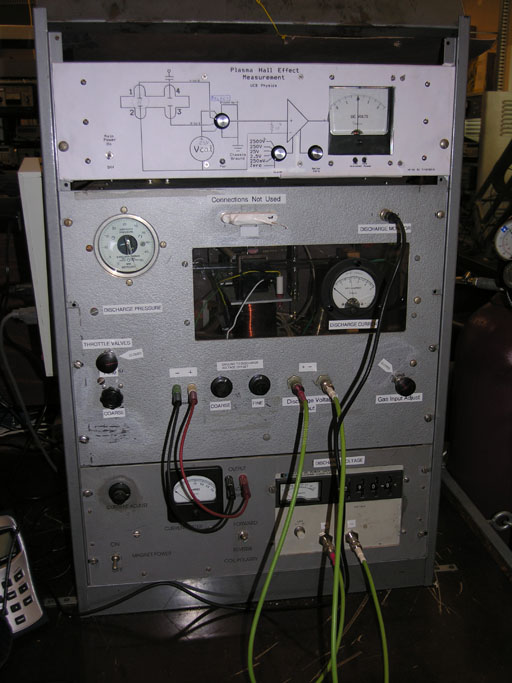
\includegraphics[width=\linewidth,keepaspectratio]{images/HAL_0153B.jpg}}
  \caption{Hall Effect Equipment Rack \\ \href{http://experimentationlab.berkeley.edu/sites/default/files/images/HAL_0153B.jpg}{Click here to see larger picture}}
  \label{fig:HAL_0153B.jpg}
\endminipage\hfill
\minipage{0.24\linewidth}
  \href{http://experimentationlab.berkeley.edu/sites/default/files/images/HAL_0152B.jpg}{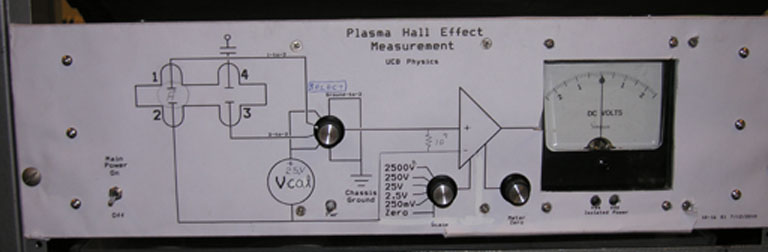
\includegraphics[width=\linewidth,keepaspectratio]{images/HAL_0152B.jpg}}
  \caption{Hall Effect Measurement Amplifier \\
  \href{http://experimentationlab.berkeley.edu/sites/default/files/images/HAL_0152B.jpg}{Click here to see larger picture}}
  \label{fig:HAL_0152B.jpg}
\endminipage\hfill
\minipage{0.24\linewidth}
  \href{http://experimentationlab.berkeley.edu/sites/default/files/images/HAL_Gas-Valves_3532-Lg.jpg}{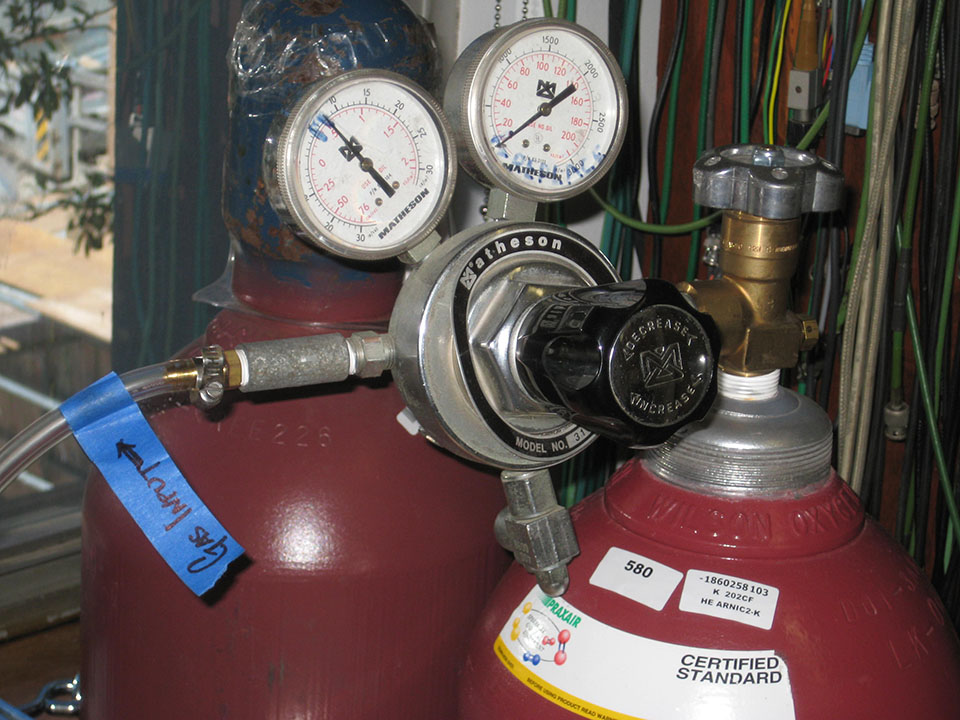
\includegraphics[width=\linewidth,keepaspectratio]{images/HAL_Gas-Valves_3532-Lg.jpg}}
  \caption{Hall Effect Tank Gas valves \\ \href{http://experimentationlab.berkeley.edu/sites/default/files/images/HAL_Gas-Valves_3532-Lg.jpg}{Click here to see larger picture}}\label{fig:HAL_Gas-Valves_3532-Lg.jpg}
\endminipage\hfill
\minipage{0.24\linewidth}
  \href{http://experimentationlab.berkeley.edu/sites/default/files/images/HAL_TC_Gauge_3533-Lg.jpg}{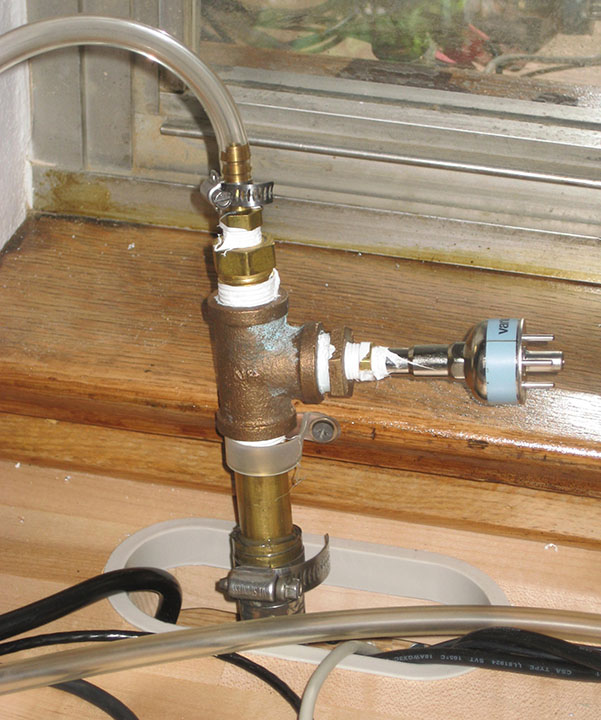
\includegraphics[width=\linewidth,keepaspectratio]{images/HAL_TC_Gauge_3533-Lg.jpg}}
  \caption{Vacuum Pressure Test TC \\ \href{http://experimentationlab.berkeley.edu/sites/default/files/images/HAL_TC_Gauge_3533-Lg.jpg}{Click here to see larger picture}}\label{fig:HAL_TC_Gauge_3533-Lg.jpg}
\endminipage
\end{figure}
\begin{figure}[!htb]
\minipage{0.24\linewidth}
  \href{http://experimentationlab.berkeley.edu/sites/default/files/images/HAL_Plasma_3570.jpg}{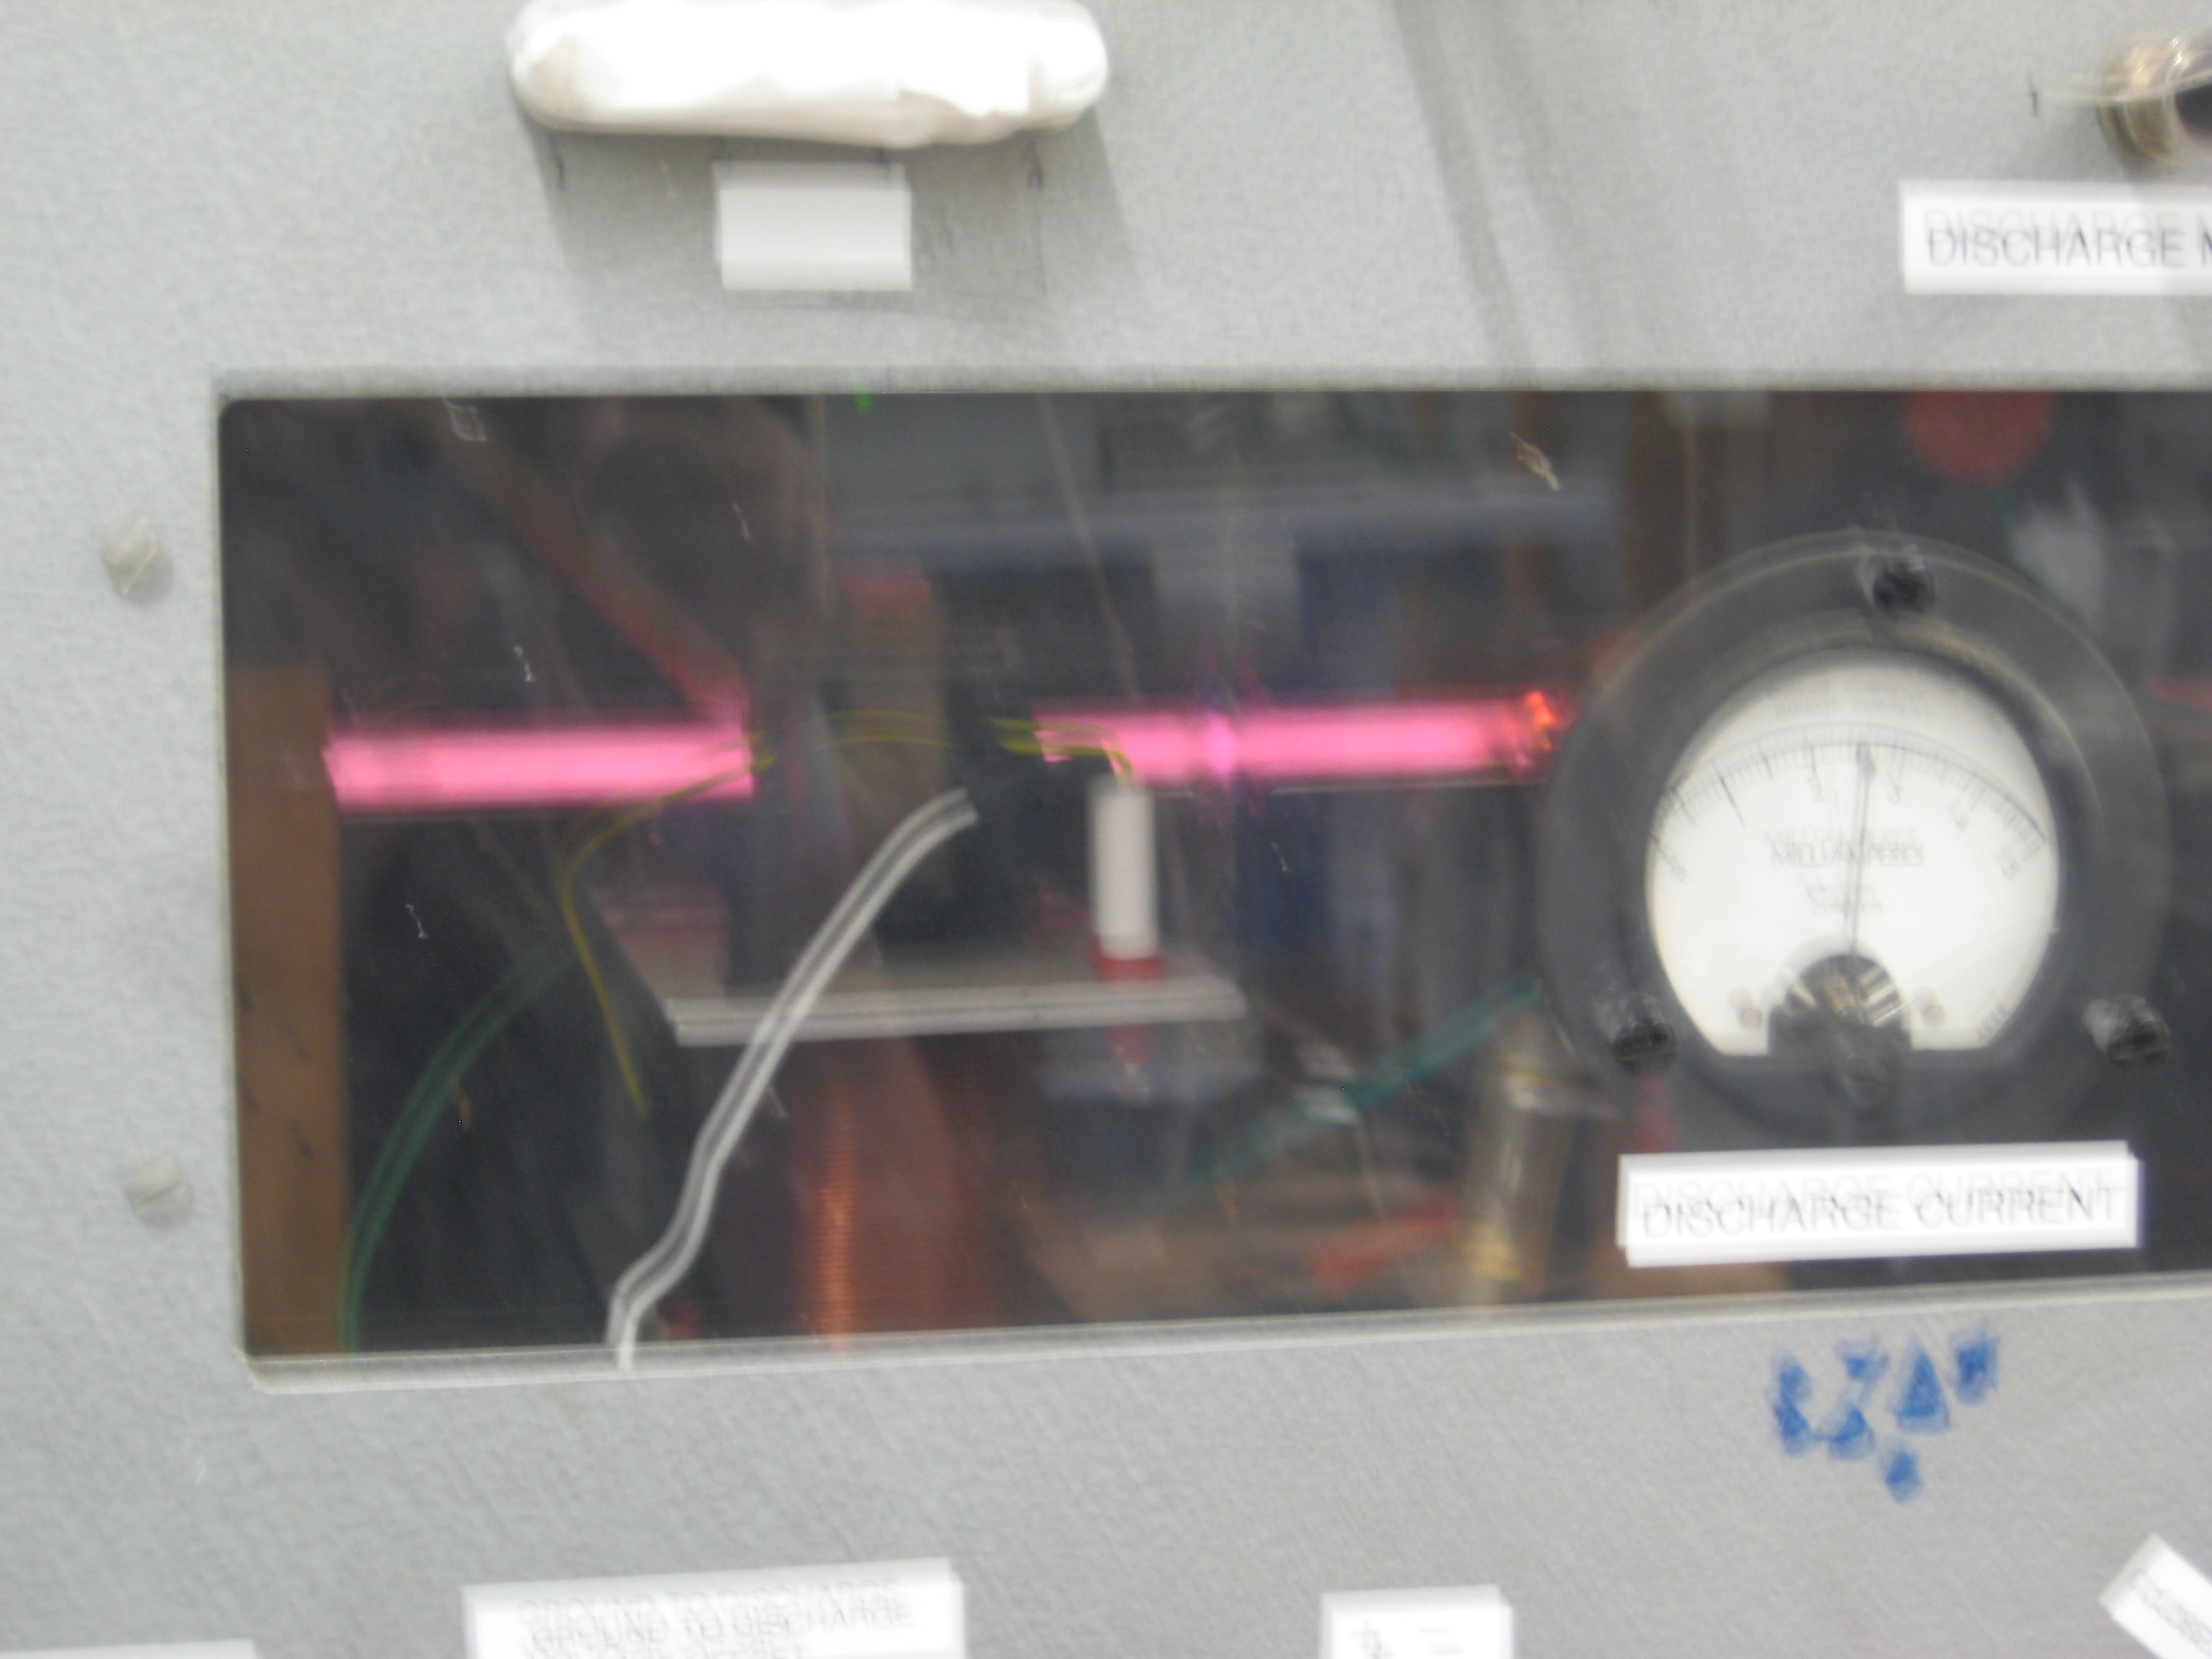
\includegraphics[width=\linewidth,keepaspectratio]{images/HAL_Plasma_3570.jpg}}
  \caption{Plasma Discharge \\ \href{http://experimentationlab.berkeley.edu/sites/default/files/images/HAL_Plasma_3570.jpg}{Click here to see larger picture}}\label{fig:HAL_Plasma_3570.jpg}
\endminipage\hfill
\minipage{0.24\linewidth}
  \href{http://experimentationlab.berkeley.edu/sites/default/files/images/Pump_Switch_3535-Lg.jpg}{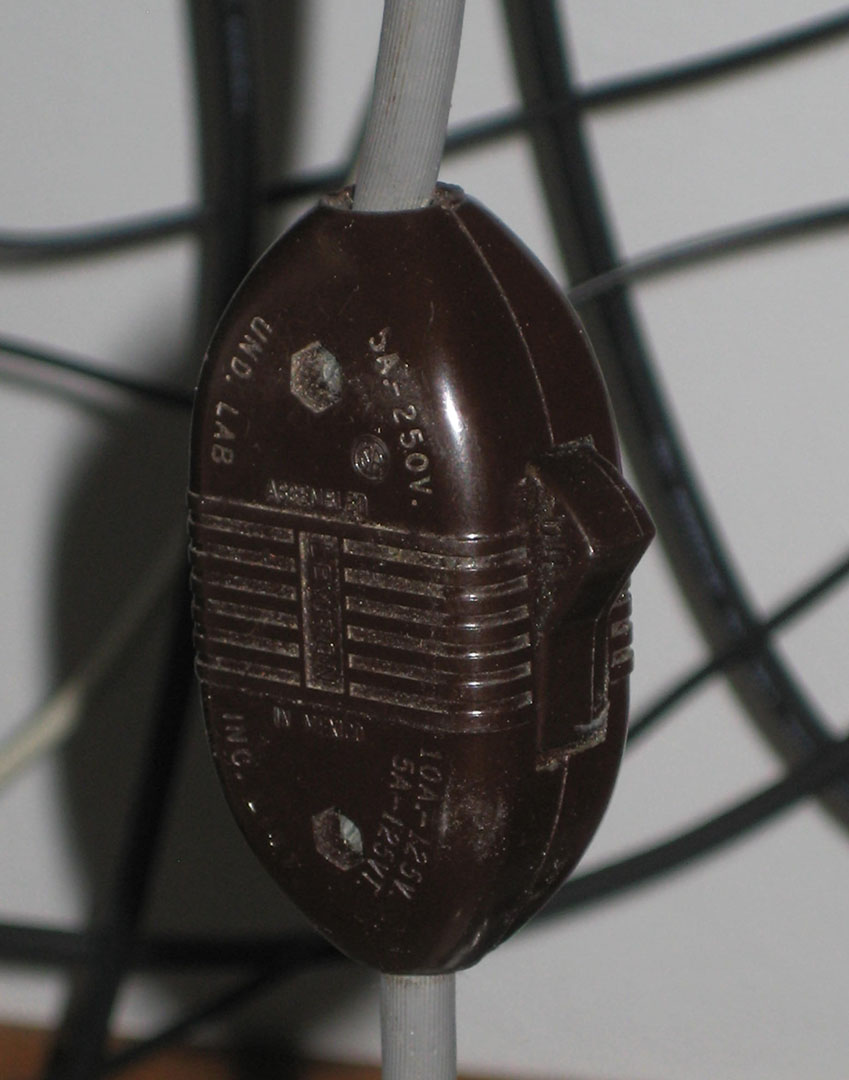
\includegraphics[width=\linewidth,keepaspectratio]{images/Pump_Switch_3535-Lg.jpg}}
  \caption{Vacuum Pump On/Off Switch under bench \\ \href{http://experimentationlab.berkeley.edu/sites/default/files/images/Pump_Switch_3535-Lg.jpg}{Click here to see larger picture}}\label{fig:Pump_Switch_3535-Lg.jpg}
\endminipage\hfill
\minipage{0.24\linewidth}
  \href{http://experimentationlab.berkeley.edu/sites/default/files/images/HAL_3510.jpg}{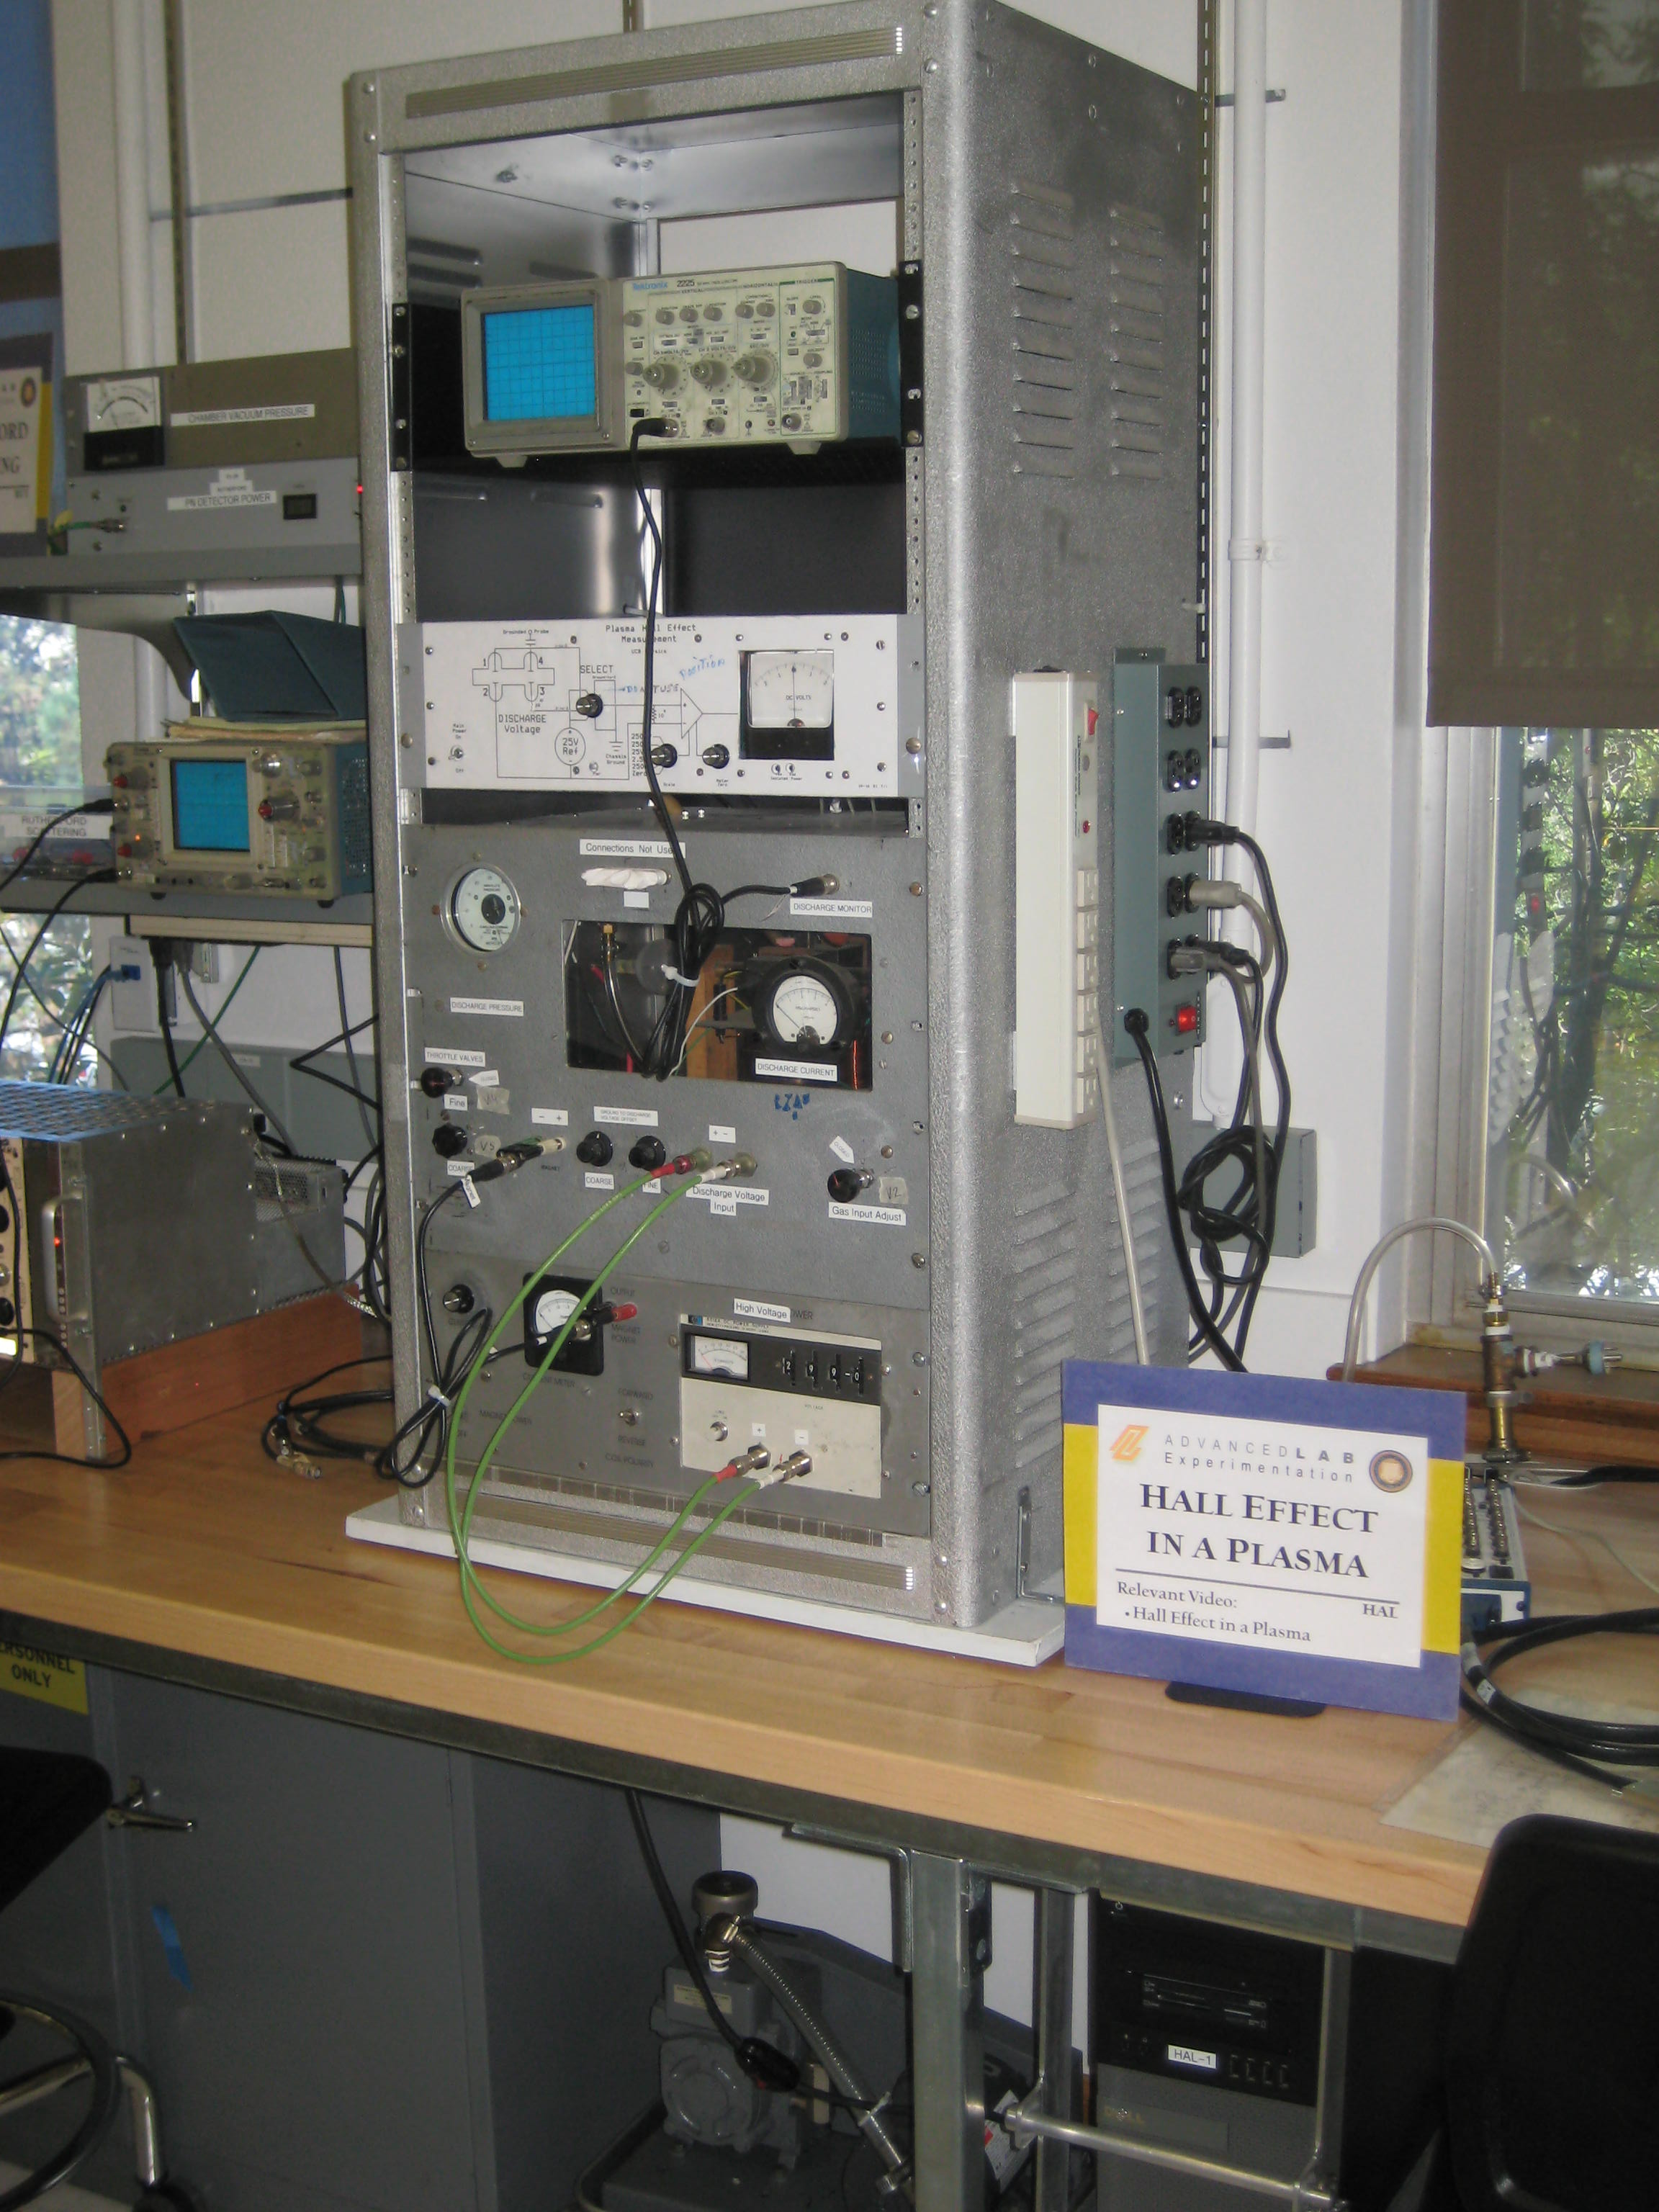
\includegraphics[width=\linewidth,keepaspectratio]{images/HAL_3510.jpg}}
  \caption{Hall Effect Rack Experiment Area \\ \href{http://experimentationlab.berkeley.edu/sites/default/files/images/HAL_3510.jpg}{Click here to see larger picture}}\label{fig:HAL_Plasma_3510.jpg}
\endminipage\hfill
\minipage{0.24\linewidth}
  \href{http://experimentationlab.berkeley.edu/sites/default/files/upimages/2_eye-wear-face.jpg}{
\includegraphics[width=\linewidth,keepaspectratio]{images/2_eye-wear-face.jpg}} \\
  \textbf{Wear Your Eye Safety Glasses}
  \label{fig:2_eye-wear-face.jpg}
\endminipage
\end{figure}

\section{Before the 1st Day of Lab}
\label{sec:BeforeFirstDay}

\textbf{Complete the following before your experiment's scheduled start date:}

\begin{enumerate}
    \item \emph{\textbf{Note: In order to view the private Youtube videos hosted by the university, you must be signed into your berkeley.edu Google account.}} \\
    View the \href{http://youtu.be/iZkOlZDyb2U}{\textbf{Hall Effect in a Plasma video}}.

    \item Complete the \href{http://experimentationlab.berkeley.edu/HALPreLab}{\textbf{HAL Pre Lab and Evaluation}} sheets. Print, fill it out, turn in your answers with the report. The Pre-Lab must be printed separately. Discuss the experiment and pre-lab questions with any faculty member or GSI and get it signed off by that faculty member or GSI. Turn in the signed pre-lab sheet with your lab report.

    \item Read about magnetic field \href{http://experimentationlab.berkeley.edu/hysteresis}{\textbf{Hysteresis}}.

    \item \emph{Check points are examination points that are placed in this lab where you must STOP and call a GSI or professor to make sure you understand what's expected. There could  be multiple check points throughout your lab so make sure you don't skip them since there is a \href{http://experimentationlab.berkeley.edu/halcheckpoints}{\textbf{sign off sheet}} that must be turned in with your lab report.}

    \item Last day of the experiment please fill out the \href{\ExperimentEvaluation}{\textbf{Experiment Evaluation}}

    \item Read W. B. Kunkel ``Hall Effect In A Plasma'', this should be your primary resource.

\end{enumerate}

\noindent\textbf{Suggested Reading:}

\begin{enumerate}
    \item W. B. Kunkel, ``\href{http://physics111.lib.berkeley.edu/Physics111/Reprints/HAL/Kunkel_HAL.pdf}{\textbf{Hall Effect In A Plasma}}'', America Journal of Physics 49, 733 (1981). \href{http://physics111.lib.berkeley.edu/Physics111/Reprints/HAL/Kunkel\_HAL.pdf}{\textbf{Searchable Page}}

    \item Golant, V.E. and et al. ``\href{http://physics111.lib.berkeley.edu/Physics111/Reprints/HAL/V.\%20E.\%20GOLANT/Ch.\%205\_Distribution\%20function\%20of\%20charged\%20particles\%20in\%20electric\%20field\%20pg.\%20108-154.pdf}{\textbf{Chapter 5}}, \href{http://physics111.lib.berkeley.edu/Physics111/Reprints/HAL/V.\%20E.\%20GOLANT/Ch.7\_Transport\%20processes\%20in\%20plasma\%20without\%20magnetic\%20field\%20pg\%20181-240.pdf}{\textbf{Chapter 7}}, \href{http://physics111.lib.berkeley.edu/Physics111/Reprints/HAL/V.\%20E.\%20GOLANT/Ch.\%208\_Motion\%20of\%20charged\%20plasma\%20particles\%20in\%20magnetic\%20field\%20pg\%20241-279.pdf}{\textbf{Chapter 8}}, and \href{http://physics111.lib.berkeley.edu/Physics111/Reprints/HAL/V.\%20E.\%20GOLANT/Symbols\_pg\%20xi-xvi.pdf}{\textbf{Symbols}}.'' \emph{Fundamentals of Plasma Physics}, Wiley, New York (1980).

    \item M. N. Hirsh, and J. J. Oskam, eds., ``\href{http://physics111.lib.berkeley.edu/Physics111/Reprints/HAL/Gaseous\%20Electronics\_HirshnOskam\%20ch2.pdf}{\textbf{\textbf{Ch. 2 Glow Discharges at DC and Low Frequencies}.}}'' \emph{Gaseous Electronics,} Vol 1. Academic Press, New York (1978). \emph{\textbf{A good book on Plasma Discharge structures.}}

    \item Lyman Spitzer, \emph{\href{http://physics111.lib.berkeley.edu/Physics111/Reprints/HAL/SPITZER/Physics\%20of\%20Fully\%20Ionized\%20Gases.pdf}{\textbf{Physics of Fully Ionized Gases}}.} 2nd Ed., Wiley, New York, (1962). A short and very readable introduction to plasma physics (this is a simple general reference to read), which \textbf{should be read to understand the basic concepts of Plasma discharges.}

    \item Read about Striations; A.V. Nedospasov, ``\href{http://physics111.lib.berkeley.edu/Physics111/Reprints/HAL/04-Striations.pdf}{\textbf{Striations}}'', Soviet Physics Uspekhi 11, 174-187 (1968).

    \item \href{http://physics111.lib.berkeley.edu/Physics111/Reprints/HAL/The\%20Hall\%20Effect\_Melissinos-2nd-Ed.pdf}{\textbf{\textbf{Hall Effect, Melissionos 2nd ed}.}} 

\end{enumerate}

\noindent\textbf{Index to the full Hall Effect Reprints List} \href{http://physics111.lib.berkeley.edu/Physics111/Reprints/HAL/HAL\_index.html}{\textbf{Hall Reprint List}}

\noindent Reprints and other information can be found on the \href{\LabReprints}{\textbf{Physics 111 Library Site}}

\noindent More \hyperref[sec:References]{References}

You should keep a laboratory notebook. The notebook should contain a detailed record of everything that was done and how/why it was done, as well as all of the data and analysis, also with plenty of how/why entries. This will aid you when you write your report.

\section{Objectives}

\begin{itemize}
    \item Learn what real experimental physics is about

    \item Learn the synergy between experimental and theoretical work

    \item Learn to use pieces of equipment that are commonly used in research

    \item Learn how measurements are performed, analyzed, and interpreted.

    \item Learn how to present your work and results

    \item Learn problem solving strategies

    \item Learn how to manage and organize your time

    \item Understand how we measure the Hall effect in Plasma

    \item Measure the discharge current as a function at the high voltage at different constant pressures.

    \item Measure the discharge voltage over the high voltage at different constant pressures.

    \item Study the limits of the magnitude of the applied magnetic field over the different currents supply to the coils.

    \item Understand the what is hysteresis  and how it contributes to our experiment.

    \item Measure the hall voltage as a function of the magnetic field.

    \item Apply data analysis to find any source of error and explore them.

    \item Understand and work out relations among Plasma parameters

    \item Calculate and explain the characteristic qualities of the electron gas such as drift velocity, electron density, collision frequency, etc..

    \item Measure and explain other relevant parameters and quantities that you find relevant to this lab.

\end{itemize}

\section{Introduction}

In low-density plasmas, such as the positive columns of glow discharges, the Hall effect is large and easily observable. In this experiment the Hall voltage across a helium discharge column is determined as a function of magnetic field, discharge current, and gas pressure. Electron drift velocities and densities are inferred from measurements of electrical parameters. A measurement of the resistance permits evaluation of the collision frequency of the electrons. The electron temperature can be calculated.

\section{The Hall Effect}

To measure the Hall effect in a conductor we apply both electric and magnetic fields. The analysis is simplest if we take care to apply them perpendicular to each other. In the most common Hall effect geometry, we measure the current that flows in the direction of the applied electric field. We confine the carriers in the direction perpendicular to the electric field, establishing a boundary condition that this transverse current is zero. To analyze the magnitudes of the various currents and voltages that are developed in steady-state, we use some simple force balance considerations.

In thinking about the electrons in a plasma, we should be careful about the distinction between the velocity of individual electrons, $\vec{v}$, and the drift velocity of an ensemble of electrons $\overrightarrow{\Delta v} \equiv \langle\vec{v}\rangle$. Before we apply any fields, the electrons are moving randomly at a high speed that reflects their temperature. The average velocity of the ensemble is zero. When we apply the longitudinal electric field, the ensemble will move in the direction of the applied force, at a drift velocity that is in general much slower than the mean thermal velocity. To determine the drift velocity, we consider what happens to an electron during its motion between collision events. During this time it experiences the electric force,
\begin{equation}
    \vec{F}_E = q \vec{E},
\end{equation}
where $q = -e$ for our problem. If the velocity of the electron just after its last collision is $\vec{v}$, then its velocity just before the next collision is $\vec{v} + \overrightarrow{\Delta v}$, where
\begin{equation}
    \overrightarrow{\Delta v} = \frac{\tau q}{m}\vec{E}.
\end{equation}
In the equation above, $ \tau$ is the mean free time. It is also common to relate the drift velocity to the collision frequency, $ \nu$, which is just reciprocal of $ \tau$ (make sure you can see the difference between $\vec{v}$ and $\nu$ in the typography!):
\begin{equation}
    \overrightarrow{\Delta v} = \frac{q}{m \nu}\vec{E}.
\end{equation}
Next, we average $ \vec{v} + \overrightarrow{\Delta v}$, over many collisions. As we assume that the initial velocity is random, so it's zero, then the average velocity is just given by $ \overrightarrow{\Delta v}$.

The effect of the magnetic field on the electrons is a little bit trickier. In the absence of an electric field, the velocities are random, and the B field has no net effect. In other words, electrons are equally likely to be curving one way as the other. However, in the presence of drift induced by the electric field, there will be a time-averaged magnetic force.
\begin{equation}
    \vec{F}_{M} = q \overrightarrow{\Delta v} \times \vec{B}.
\end{equation}\label{eq:time-averaged-magnetic-force}
Let's choose coordinates such that the magnetic field is along the $z$-axis and the electric field is along the $x$-axis. Under such conditions, electrons will drift in the $x$-direction under the influence of the applied field. The force caused by the magnetic field will therefore be in the $y$-direction. Note that neither $E$ nor $B$ will yield a force in the $z$-direction. As stated above, in the most common Hall geometry, we confine the electrons so that the net current in the $y$-direction is zero. As a result of this boundary condition, an electric field develops that balances the magnetic force on the drifting electrons. The quantitative study of the Hall effect is all about the ratio of this electric field to the applied B field.

The magnetic force on the drifting electrons is obtained by substituting the drift velocity into the Lorentz force equation,
\begin{equation}
    F_y = -\frac{q^2E_xB_z}{m \nu} .
\end{equation}
To maintain a condition of zero current flow in the $y$-direction, an electric field given by,
\begin{equation}
    E_y = \frac{qE_xB_z}{m \nu} ,
\end{equation}
must be established. Since physicist's love dimensionless quantities, we should consider the ratio,
\begin{equation}
    \frac{E_y}{E_x} = \frac{qB_z}{m \nu} ,
\end{equation}
which is known as the Hall angle. Notice that familiar combination of parameters appears here. Yes, qB/m is just the cyclotron frequency, which is 1.8 $\times 10^{11}$ Hz for a magnetic field of 1 Tesla. A nice expression for the Hall angle is then,
\begin{equation}
    \Theta_\textrm{Hall} = \omega_c \tau .
\end{equation}
The analysis of the Hall effect that we have done is valid when the cyclotron frequency is smaller than the collision frequency. In this regime, the electron's motion is interrupted by collision before it can complete a cyclotron orbit.

To learn as much as we can about conduction in the plasma we should measure the longitudinal current as well as the Hall angle. The electric current density $\vec{j}$ is given by,
\begin{equation}
    \vec{j} = q n \overrightarrow{\Delta v}.
\end{equation}
The resistance of plasma, which we call $\rho$, is the ratio of this current to the longitudinal electric field, or,
\begin{equation}
    \rho = \frac{E_x}{j_x}.
\end{equation}
In the longitudinal (unconfined) direction, the current is determined by balancing the force due to the applied electric field and the frictional force. This balancing act yields the following expression for the resistance,
\begin{equation}
    \rho = \frac{m\nu}{q^2n}.
\end{equation}
If we can measure both the Hall angle and the resistance, this gives us two independent observables. In general, a conductor under study has four independent parameters: the density, charge, mass, and scattering rate of the mobile charged species. In the case of our plasma, the current is carried by electrons, and therefore the mass and charge are known to us. In this case our two independent observables are sufficient to determine the remaining two parameters - the density and collision rate of the electrons.

\section{Hall Effect in Glow Discharge Columns}

In the discussion above we assumed that the density of electrons was uniform in space. For homogeneous systems in thermal equilibrium this is a reasonable assumption. However, this is not case for the plasma. The free electrons in the plasma are produced in ionizing collisions with gas atoms or molecules confined at a low pressure in a long narrow discharge tube. At the low current densities under consideration here, recombination of the charged particles takes place almost exclusively at the tube walls. This means that the electrons (and positive ions) produced in the gas must find their ways to the walls before they disappear. The resulting electron density distribution is not uniform, but has a maximum in the center of the tube, and falls nearly to zero at the walls. When a transverse magnetic field is applied the electrons are redistributed to counteract the Lorentz force, and a Hall field is set up. This Hall field is not uniform across the plasma. Therefore, the Hall voltage, which is the integral of the Hall field, is not simply the product of the Hall field and separation of the electrodes. However, it turns out that Hall voltage that you actually measure is, in fact, exactly one-half the expected value, for the case of slab geometry. The proof of this can be found in the book by Golant et al (See \hyperref[sec:BeforeFirstDay]{Golant Reading Materials}).

Armed with this knowledge, you can use the measured Hall voltage and longitudinal current density to obtain the electron density and scattering rate. As a quantitative example, we can operate a glow discharge at a current density of 10 A/m$^2$ in a mixture of 1\% argon in helium at $p$ = 30 torr pressure and find a Hall field $E_H$ = 300 V/m when $B$ = 100 gauss, and an ohmic field $E_o$ = 5000 V/m. This tells us that the electron drift speed is $u_e$ = 30,000 m/sec, and therefore the free electron density is approximately $n_e = 2 \times 10^{15}$ m$^{-3}$. The gas density calculated from the ideal gas law, on the other hand, is $N_g = 10^{24}$ m$^{-3}$, so that the degree of ionization $n_e/N_g$ is only about $2 \times 10^{-9}$. Note: Measure the distance between the pole pieces!

While we have learned a lot, notice that we don't obtain any direct information about the thermal velocity of the electrons in the plasma. However, we can make some indirect inferences. We know the electron collision frequency and the density of the atoms that the electrons are colliding with. According to kinetic theory, the collision frequency is related by the scattering cross section for momentum transfer, that is,
\begin{equation}
    \nu \cong N_g \sigma v .
\end{equation}
where  \textbf{$\sigma$}  is cross section, and $v$ is the speed of electron (More in depth explanation in W. B. Kunkel). Where In our experiment using He gas the cross section is approximately equal to $3.8 \times 10^{-20}$ m$^2$. Using this value for cross section and the expression above, the mean electron speed and hence the mean electron energy, or temperature can be estimated. The collision rate equation gives the average speed and the temperature is related to the mean square speed. For the MB distribution the mean square speed is not equal to the square of the average speed and you should take this factor into account. See Kittle for discussion on this point.

If you do your calculations correctly, you should obtain some rather large electron speeds and temperatures. The electron temperature $T_e$ can exceed 10,000K. You might be wondering if you should keep your hands off the glass tube that encloses the plasma. In fact, the glass is only barely warm to the touch. What is this telling about the nonequilibrium state in the plasma? A hint is that it should be related to the efficiency of energy transfer from the electrons to the He atoms. Can you explain why the thermal contact between the free electrons and the background gas is so weak? It can also be shown that the energy in random motion of the free electrons has an upper bound given by
\begin{equation}
\label{eq:energy}
    \textrm{Energy} = \left ( \frac{1}{2} \right ) m \left \langle v^2 \right \rangle < \left ( \frac{1}{2} \right ) M_g \Delta v^2
\end{equation}
where $ \Delta v$ denotes again the \textbf{drift} speed and $M_g$ is the mass of the gas atom or molecule. The upper limit is reached when electron energy loss due to inelastic collisions (excitation and ionization) is negligible compared to that caused by elastic collisions. A substitution of the mass of the helium atom and the electron drift speed of our example into eq.~\eqref{eq:energy} yields an energy upper limit of 18 eV.

Although 1 eV is very much higher than the thermal energy of the gas, it is much lower than most ionization energies. The ions produced in our gas mixture are primarily argon, which has an ionization energy of 15.8 eV. How can ionization take place when the mean electron energy is much lower than the energy required to liberate an electron from the gas atoms? You may have noticed that in the steady state, a local rate balance between ionization and recombination at an electron temperature of 10,000K and at the densities quoted here, the degree of ionization should be very high rather than the very low level observed. The explanation is that the loss of ions in these discharges at low gas pressures is controlled by transport to and recombination at the relatively cool walls. This is a second and equally important process causing pronounced deviations from equilibrium conditions.

The matter of energy balance and of charged particle production, transport, and loss are thoroughly discussed in the texts on ionization phenomena in gases. The steady state condition for the column of a glow discharge is a delicate balance between several non equilibrium processes. It is not surprising that such columns display a variety of oscillations and non-uniformities that sometimes interfere with our Hall effect observations and therefore deserve some attention.

\textbf{This is a checkpoint and a great time to stop and think about the physics at play. Discuss the following questions with you partner and once you feel you have a better understanding of what is happening, call over a GSI to sign you off:
How can ionization take place when the mean electron energy is much lower than the energy required to liberate an electron from the gas atoms?}

\section{Instabilities, Oscillations, and Striations}

Plasmas are in general unstable entities. If plasmas were intrinsically stable, plasma fusion reactors could already be supplying commercial electricity, but they are not. The stability of a plasma is dependent on almost anything imaginable, not only the obvious: current, voltage, pressure, magnetic field and mass flow rate; but potentially also the non-obvious: contaminant gases, ambient temperature (untested), ambient light (not observed), and time (very important). It is characteristic of all plasmas that they can support many types of waves. Some of these waves grow spontaneously from thermal fluctuations to large amplitudes. In that case they are called instabilities. Most instabilities in our discharge are driven by the electric current, somewhat like whistle tones are excited by air streaming through pipes. A small change in current or in gas density can change the oscillatory behavior completely. Therefore, pay attention and don’t change the gas pressure or flow in the middle of taking a set of data.

You should have read the articles on \href{http://physics111.lib.berkeley.edu/Physics111/Reprints/HAL/04-Striations.pdf}{\textbf{Striations}}

Observations reveal that oscillation frequencies are in the multi-kilohertz range, with amplitudes sometimes in excess of a few volts. It is therefore important that measuring devices be protected by low-pass filters consisting of RC input circuits with about 0.2 sec time constants. Quiescent (oscillation-free) operation is a necessity for all measurements. You may have to invest some time finding a stationary state, by varying the current, gas pressure, and flow rates. Patience is needed. The gas is a mixture of helium with 1\% of argon and 0.1\% of nitrogen. The argon is most easily ionized and supplies most of the free electrons, while the nitrogen is added to make the entire mixture relatively insensitive to contamination by air and other residual impurities. A small flow rate is required to keep the mixture constant. Too rapid a flow causes turbulence in the gases.

Under many operating conditions, particularly at the lower pressures, a striking stationary structure appears in the visible glow consisting of alternating bright and dim regions or striations. These can be considered as large-amplitude ionization waves. The amplitude modulation of the luminous intensity, which may approach 100\%, is much larger than the axial variation of electron density which rarely exceeds 20\%. It turns out to be primarily caused by the variation in the tail of the electron energy distribution which is responsible for most of the visible radiation. The effect on our Hall voltage is therefore only minor, and we can ignore the presence of stationary striations for our purposes. The effect on $E_o$ is also minor if the distance between probes is made large enough to permit averaging over several wavelengths of these striations.

\section{Apparatus and Equipment}

\begin{enumerate}
    \item The equipment required for this experiment is contained in the Plasma Hall Effect rack. The labels on the rack controls are intended to faithfully reflect the descriptions in this text, though schematic labels in the text and on the gas flow diagram are NOT attached to the physical valve handles. Rather, physical valve handles are labeled on the rack corresponding to their functional description, such as ``Gas Input Adjust'' (for valve v2).

    \item The gauss meter, an oscilloscope (any scope with a 1M input will do), the gas supply cylinder (right side) and the vacuum pump (under the bench) are the required components that are external to the Plasma Hall Effect rack.

    \item The schematic diagrams of the gas flow system, the plasma electrical measurement system (including supplies, meters, and the discharge tube), and the magnet circuits, are included in the following sections. These systems are functionally independent though they all affect the plasma and its characteristics.

    \item The impedances of the supplies and the meters are explicitly identified to assist the experimenter in identifying potential measurement errors. Like most physical experiments utilizing electrical measurements, the results depend on the interaction of a non-ideal physical construction (the discharge tube containing the plasma) with non-ideal electrical instruments. The thoughtful experimenter is mindful of these interactions, taking care to minimize the deleterious effects on the measurements. The instruments perturb the physics.

\end{enumerate}

\section{Equipment Notes}

\subsection{General, the gas and the plasma}

The vacuum and gas supply system, including the line between the inflow needle valve and the high-pressure regulator, is leak-free enough to permit a base vacuum pressure below 2 mm of mercury (2 Torr) pressure. However, due to back-pressure after shutting off the pump and closing the valves, pressure will build up in the system at a rate of $\sim$1 Torr per 11 minutes, which is insignificant. So, when shutting off the system and returning at a later time, don't be alarmed if their is a high pressure reading on the gauge. Glow discharges are sensitive to contamination, especially by organic vapors, and this plasma discharge tube is no exception. Considerable flushing (flowing gas through the discharge tube with the plasma established) helps establish a stable plasma discharge characteristics. The longer the duration of a plasma discharge, the more stable and reproducible the discharge conditions become and the wider the discharge operating range in pressure (up to 30 Torr) and current (below 0.3 mA).

The settling time of the plasma that is to a stable current-voltage, and noise operating point may be several minutes. As a result of this long settling time, the plasma control parameters: pressure, flow rate, and discharge voltage need to be changed slowly while monitoring the plasma response parameters discharge current, plasma physical appearance (striations), discharge current/voltage noise at the discharge monitor. If the control parameters are changed too quickly, one of the most common and annoying results is that the discharge extinguishes and the control parameters need to be returned to a starting point.

As a guideline, changes to pressure should be slower than 1 Torr every 10 seconds and the voltage changes 100V in 5 seconds.

The color of the glow is sensitive to gas composition, which for the helium/argon/nitrogen mixture used in this experiment, is pink. Although the system is leak tight, it is desirable to keep the gas pressure upstream of the input valve (labeled ``Gas input adjust'') slightly above atmospheric pressure in order to prevent air from entering the gas system between the input valve and the gas regulator. This higher pressure has the disadvantage of operating with a large pressure drop across the input valve, thereby making the plasma discharge pressure very sensitive to the setting of this valve. On the other hand, once the input valve conductance is set, a nearly constant gas flow rate has been established.

\subsection{How to set a gas pressure and gas flow rate}

The drawing below (see Fig~\ref{fig:680px-Hall_diagram}) illustrates the complete plasma discharge gas flow system, which is similar to other low pressure gas delivery systems. A gas source (He/Ar/N tank) supplies gas at about 5 psi ($\sim$1000 Torr  at p2 where units are kg/cm$^2$). The discharge tube pressure (p3) is nominally 10-30 Torr so that valve v2 conducts gas a nearly constant rate determined by the $\sim$1000 Torr differential pressure valve v2’s conductance G2. G2 is a needle valve with relatively low conductance. This procedure establishes a constant gas flow rate into the discharge tube.

The rotary-vane vacuum pump has a very high evacuation capacity and would require a significant gas flow through v2 to achieve the proper discharge pressure at p3. It is common practice to insert a ``throttling'' valve (v4 \& v5) between the vacuum pump and the discharge tube to allow reduce the effective evacuation capacity, effectively throttling the vacuum pump. The throttling valve allows a pressure differential between the vacuum pump ($\sim$0 Torr) and the discharge tube (p3, 10-30 Torr).

When the pressure in the discharge tube is stable, the gas inflow equals the gas outflow. With valve v5 closed then (p2-p3) $\times$ G2=(p3-0) $\times$ G4. With p2 = 1000 Torr and p3 = 10 Torr, the ratio of valve conductance, G4/G2 $\sim$ 100. That is, the conductance of valve v4 has to be 100 times that of valve v2, or practically stated, needle valve v2 will be almost closed while valve v4 will be significantly open.

To avoid damaging the valves in the Hall plasma system and as general information, some guidelines should be observed. All the accessible valves are right handed, that is they close when turned clockwise. Only hands without tools should be used to adjust valves. Valves v2, v3, and v5 can be closed with one finger and a thumb. Valve v1, on the top of the gas cylinder requires a full grip to open and close (and considerable torque), but only needs to be opened and closed about 1/4 turn. It is very important to close v1 when the experiment is not in use. Each gas cylinder is a ten-year supply. So why is there a spare cylinder of gas?

The gas regulator, r1, attached to the gas cylinder, and controlled by the large black knob, does not normally need to be adjusted. When v1 is open, p1 should indicate 100-2000 psi and p2 indicate 4-6 psi. If for some reason p2 is not 4-6 psi when v1 is open, first tap on the regulator r1 and gauge p2 with your knuckle. If p2 still does not indicate a pressure of 4-6 psi, the pressure at p2 may be increased by slowly turning the black knob (r1) clockwise. If the pressure is too high, a counter-clockwise rotation of the black knob of r1 will reduce the pressure at p2 ONLY if the gas has someplace to go. Therefore, before turning the black knob to adjust p2, it is required to have the vacuum pump on and v2 and v4 both open 1/4 turn.

There are two techniques for establishing a flow and a pressure with this gas flow configuration. The first technique is the more traditional of the two: set flow (v2) then set pressure (v4) at constant flow. The second technique is a non-constant flow required to reach discharge pressures in the 12-35 Torr range and requiring a higher conductance than v4 can provide using the first technique. The second technique requires that the discharge is established AND then the flow AND pressure are increased.

With v5 and v2 closed, open v4 3 turns (3.5 turns is all the way open) and wait about 30 seconds, p3 should read about 1 Torr.

Technique 1: Open v4 by 1/2 turn, open and adjust v2 until p3, ``discharge pressure'', indicates 10 Torr. This is the low gas flow set point. Do not change v2 as the flow rate is set. Open v4 2 turns and enable the discharge voltage.

Technique 2: Open v4 3 turns, open and adjust v2 until p3, ``discharge pressure'', indicates 15 Torr. This is the fixed conductance point of v4. Do not adjust v4. The gas flow through v2 and v4 is proportional to p3/G4. Enable the discharge voltage. To increase the discharge pressure, open v2 which will increase p3 and the flow rate proportionally.

\textbf{This is a checkpoint and a great time to stop and think about the physics at play. Discuss the following questions with you partner and once you feel you have a better understanding of what is happening, call over a GSI to sign you off:
Establish a stable plasma flow by following one of the two techniques listed above. Which technique do you prefer to use at 30 Torr?}

\begin{figure}[h]
    \centering
    \href{http://experimentationlab.berkeley.edu/sites/default/files/images/680px-Hall_diagram.png}{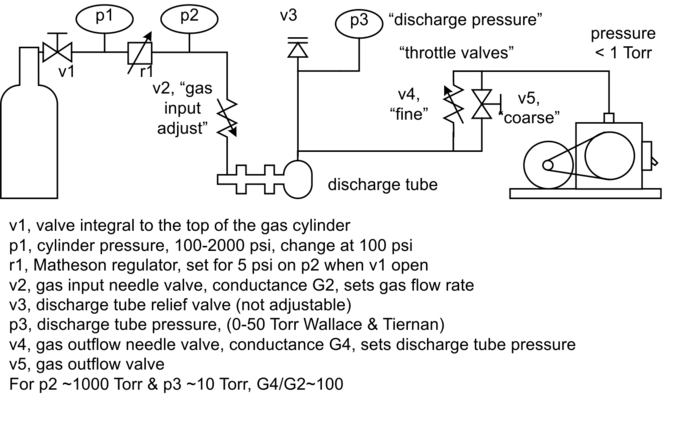
\includegraphics[width=0.8\linewidth]{images/680px-Hall_diagram.png}}
    \caption{Plasma Discharge Gas Flow System}
    \label{fig:680px-Hall_diagram}
\end{figure}

\subsection{How to set a gas pressure}

1st pump out the system with the coarse pump-out valve open, on the left side of rack, then open the Gas Input Adjust valve on the right side of rack one turn, with the main gas cylinder tank closed. When the vacuum meter reads near zero, close the main coarse pump-out valve (Throttle Coarse) and open all the way the needle valve (Throttle Fine) on the pump-out side of the system (NOTE: these two valves are in parallel). Now open the cylinder tank main valve and adjust the pressure meter to read above 1 lb. Time to adjust the gas inlet valve on the right side of rack to the lowest pressure you want for the first pressure set point. Now adjust the pump-out needle valve for the other pressures you want for the experiment.

Acceptable discharge conditions -- the oscilloscope showing no fluctuations larger than 0.1 V -- can be produced at pressures between 3 torr and 35 torr, with currents between 0.5 and 2 mA. At the low-pressure end of this range stationary striations are very pronounced and can interfere with the measurements. So keep the current low if possible. Some modest stationary striations (relatively small intensity modulation) are visible over most of the range but are mild enough not to distort the reading of $E_o$ and $E_H$ by more than 10\%. The conditions can be kept reproducible by maintaining a very small flow rate which replaces the gas content of the tube about every five seconds.

It is essential that the discharge power supply have a floating ground connection so that the Hall probes can be kept close to ground potential by means of the potentiometer bridge arrangement. \emph{\textbf{See the Circuit Diagrams}}. The reason for this requirement is the following: the effective contact impedance between a small probe and a low density plasma is several mega-ohms. It is also nonlinear, increasing rapidly when drawing primarily ion current from the plasma. The leakage resistance of standard cable connectors and feed-through insulators is between $10^9$ and $10^{10}$ ohms. If either the cathode or anode were at ground potential, the probes and Hall measuring circuits would be at positive or negative potentials of about one kilo-volt, and unwanted probe currents would be quite large. The biasing potentiometer, which adjusts the potential of the probes, needs adjustment each time a discharge parameter is changed. When this precaution is taken, good linear relationships are found between the Hall probes and the B-field up to at least 200 gauss in either direction. Observed deviations from the linear relationship given in eq.~\eqref{eq:time-averaged-magnetic-force} at higher magnetic fields are presumably caused by magnetically induced distortions of the discharge. When the field is too strong the visible appearance of the glow between the pole faces is noticeably changed, indicating excessive deviations from axial symmetry.

\textbf{This is a checkpoint and a great time to stop and think about the physics at play. Discuss the following questions with you partner and once you feel you have a better understanding of what is happening, call over a GSI to sign you off:
Locate the valves and probes from the plasma discharge gas flow system depicted above and explain how they affect the pressure in your discharge tube.}

\section{Plasma Discharge and Associated Electrical Instruments}

The discharge tube containing the plasma is powered through a 0-3 kV supply ``discharge voltage'' that is voltage referenced to the chassis (earth) ground through a resistor divider, the ground-to-discharge voltage offset. This offset voltage as well as the potentials of the discharge electrodes 1 and 3 can be measured by means of a high impedance ($10^9$ ohms, $<$ 100 pF), bipolar voltmeter with full scale voltages of 2500 V to 250 mV as illustrated below. Electrode 4 is capacitively coupled to an external oscilloscope to monitor the discharge stability via the ``discharge monitor'' port.

The voltmeter, pictured as an ideal amplifier with $10^9$ ohm input impedance, can be connected to either of 4 connections via a low-leakage current relays. One connection is to a 25 V calibration voltage. The other 3 connections are to electrodes 1, 3 and the chassis ground. The return voltage to the voltmeter, or the reference voltage, is electrode 2. Note that the connection to electrode 3 is via a $10^{10}$ resistor.

The voltmeter may be zeroed by selecting the ``zero'' range on the voltmeter range selection switch and rotating the ``meter zero'' knob. This is the only configuration in which the voltmeter should be zeroed. The discharge current should be zero during this operation.

Another point worth noting is that the discharge voltage is connected to the discharge tube via 0.5M ohms. This resistance effectively limits the discharge current to 6 mA if the plasma resistance were 0 ohms. However, as the minimum voltage across the discharge tube required to sustain plasma is about 1.5 kV, the discharge current is effectively limited to about 3 mA.

\section{Monitoring Noise in the Discharge}

\section{Procedure}

\subsection{Turning on the system}

\begin{enumerate}
    \item Check all electrical and gas flow connections. All gas valves must be closed, all electrical power off.

    \item Turn on the pump.

    \item Open the pump-out valve (Throttle Valve Coarse v5) (see Fig~\ref{fig:680px-Hall_diagram}). Vacuum gauge should go down towards 2 Torr (It may take about 2-4 whole turns). If not, call a Staff person and ask for help.

    \item Open the main valve v1 and coarse valve, this is the one to the right of p1 and p2, on He supply tank. ASK IF YOU DON'T UNDERSTAND WHAT EACH KNOB OR HANDLE DOES, OR WHAT THE GAUGES MEASURE. The high-pressure gauge, this is p1, should read between 100 and 2,000 lb/in$^2$ (psi) pressure. If the tank pressure is below 50 lb/in$^2$, get a new bottle. (Call for assistance from the staff)

    \item Close the pump-out valve (Throttle Valve Coarse, you should know this one by now). The low pressure in the discharge tube should not rise rapidly. If it does, there is a leak. Get help.

    \item Open the outflow valve (Throttle Valve Fine) 1 turn.

    \item Open the ``Gas Input Adjust'' needle valve ,VERY SLOWLY about 1/4 turn, or until pressure rise is very noticeable. At the same time, adjust the regulator valve, r1, of the gas cylinder - \textbf{set to the blue mark on the left-hand regulator gauge p2.}

    \item Adjust the pump-out needle valve (Throttle Valve Fine) to obtain steady conditions between 10 and 30 Torr pressure. At this point if your pressure can't be adjusted you may have opened v2 the ``Gas Input Adjust'' a little too much. Once a small flow rate is established it is best not to touch the input valve again, but to do all regulation with the outflow needle valve (Throttle Valve Fine). It permits much finer adjustment because the pressure drop across it is much smaller.

    \item After a few minutes of steady flow, turn on the high voltage to about 2,500 V. There will be a discrepancy between the voltage value read on the kilovolt meter and the value set on the knobs, but the turnable knobs used to set the high voltage is the true indicator of actual voltage being applied, and the meter is just a reference. There should be a glow, purplish pink in color, and the ammeter should read about 1 mA. Think about how can the pressure in the tube may affect your discharge current.

    \item Turn on the oscilloscope, to monitor the fluctuations in the plasma potential by means of the grounded probe. Under proper conditions, oscillations should be much smaller than 0.1 V, perhaps 50 mV peak-to-peak. If oscillations are too large, change the gas pressure, flow rate, high-voltage setting, etc. until quiescent operation is found. If unsuccessful, turn discharge off for one minute, then start it again. The start-up voltage may have to be higher than the operating voltage, particularly at the higher pressures. Repeat the process a few times if necessary. If oscillations are still too large, get help.

    \item If all is well, turn on the probe circuits with the voltmeter range setting at 250 V or 2500 V. Leave the magnet power off. DO NOT USE THE DVM.

    \item Adjust the discharge ground (grounded probe) with the potentiometer so that probe \#2 floats near the ground potential using dials on the front panels. First, make sure the operational amplifier is properly adjusted to give the correct reading. Set 'Scale' to zero, then adjust 'Meter Zero' until the adjacent voltmeter gives a zero reading. Set the 'Select' dial to 'Ground-to-2' and 'Scale' to the appropriate scale. Then, use the 'Coarse' and/or 'Fine' dials of the potentiometer (labeled as 'Ground to discharge voltage offset' on the front panel) to adjust the ground to probe \#2. If conditions are steady, this probe floating potential will not drift by more than a few volts (a fraction of one volt on our meter) in several minutes. Every change in conditions requires a potentiometer adjustment, however.

\end{enumerate}

\textbf{This is a checkpoint and a great time to stop and think about the physics at play. Discuss the following questions with you partner and once you feel you have a better understanding of what is happening, call over a GSI to sign you off:
Show you understand how to shut off the system completely and why it needs to be done that way. You don't have to turn off the system but simply supply your instructor with enough information to display you understand why we must take safety measurements.}

\subsection{Measurements}

\begin{enumerate}
    \item $I_d$ and $V_d$: The purpose of these first measurements is to illustrate some of the interesting properties of a plasma discharge. For a range of discharge tube pressures between 15 and 30 torr, measure the discharge current, $I_d$, and the discharge voltage, $V_d $, as a function of high voltage. The discharge voltage is given by the potential between probes 2 and 3. Note that there is a $10^{10}$ ohm resistor in series with probe 3, to keep current flow around $10^{-8}$ A. Before you take data, play around with the high voltage, discharge current, gas pressure, and gas flow, in order to get a feel for the limits on the parameters. When taking data, a typical procedure is to set the pressure to 15 torr, set the high voltage somewhat higher than it takes to keep the discharge going properly, measure the current, and record it and the voltage. Then increase the current by adjusting the high voltage, and again record the current and voltage. Repeat until you have enough points to plot a curve. Now change the pressure to 20 torr, and repeat. Continue until  6 pressure plots are obtained. Think about what you are doing, and what other data you might need. What do you need to know to go from current to current density, from power supply voltage to discharge tube voltage, etc.?

    \item $B$ vs. $I_m$: Using a gauss meter model 5180 with the HIGH VOLTAGE SUPPLY OFF, measure the magnetic field strength as a function of magnet current for both directions of magnet current flow (measure both the FORWARD and REVERSE directions of magnet current flow – just flip the COIL POLARITY switch into the correct position).

    1st = Select Auto Zero. To select AUTO ZERO operation, press the ZERO pushbutton. Unit automatically returns to normal operation. 2nd = Select Auto Range. To select AUTO RANGE operation, press the SHIFT pushbutton followed by the RANGE pushbutton. Press the SHIFT pushbutton followed by the RANGE pushbutton to exit Auto Range mode. Manual Range. Also; To select MANUAL RANGE operation, press the RANGE pushbutton. Press the UP (5) and DOWN (6) arrow pushbuttons to select ranges. Press the RANGE pushbutton to return to normal operation. For a complete Manual See [\href{http://physics111.lib.berkeley.edu/Physics111/Equipment\_Manuals/Gaussmeter5180.pdf}{\textbf{Gaussmeter}}] For an interactive Manual see [\href{http://physics111.lib.berkeley.edu/Physics111/Reprints/HAL/5180Manual.exe}{\textbf{HAL 5180Manual.exe}}] See the Circuit Diagrams for more details from the schematic. Plot $B$ as a function of $I_m$. Does the magnet display significant hysteresis? See the Hysteresis page.[\href{http://experimentationlab.berkeley.edu/Hysteresis}{\textbf{Hysteresis}}]

    Is the B-I relationship linear? In this experiment, errors owing to hysteresis are small compared to other errors. Do not spend too much time calculating and explaining them or the phenomenon of hysteresis.
    
\newpage

    \item $E_H$ vs. $B$. For a range of pressures between 15 and 30 torr measure the Hall field between probes 1 and 2 as a function of magnetic field (note that probes 1 and 2 are about 8 mm apart). Take data for the full range of magnet current. Remember to keep the probes near ground potential by adjusting the potentiometer. Plot your results for each pressure. Is $E_H$ linearly dependent on B? For the linear parts of your data (usually $B$ less than 300 gauss) calculate quantities describing the electron gas ($v_e$, $n_e$, $\nu_e$, $\langle \sigma v \rangle$, $T_e$, etc.). Are your results reasonable? How do these quantities change with pressure?

\textbf{This is a checkpoint and a great time to stop and think about the physics at play. Discuss the following questions with you partner and once you feel you have a better understanding of what is happening, call over a GSI to sign you off:
Show the $E_H$ vs. $B$ plots taken at various pressures and explain your results using the above questions.}

\end{enumerate}

\subsection{Glow Discharge Structure}

Below shows the Voltage-Current curve of self-sustaining glow discharge. Notice the Normal Glow Region which is linear. This is the region where probes 2 and 3 are located. The voltage here should be linear and constant.

\begin{figure}[h]
    \centering
    \href{http://experimentationlab.berkeley.edu/sites/default/files/images/DischargeStructure.jpg}{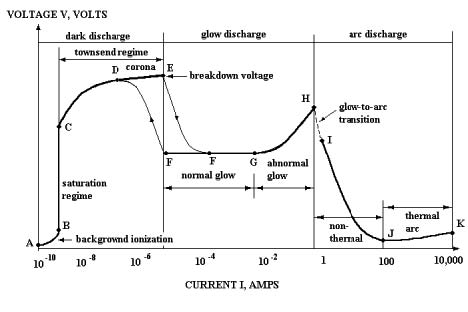
\includegraphics[width=0.8\linewidth]{images/DischargeStructure.jpg}}
    \caption{Voltage vs. Current curve of self-sustainng glow discharge}
\end{figure}

\subsection{Shutting off the system}

\begin{enumerate}
    \item Shut off the probe circuits and oscilloscope. Turn off the magnet power and discharge high-voltage power supply.

    \item Open the pump-out valve.

    \item Close the main valve on the helium gas cylinder.

    \item Open the inflow valve wide, until the high-pressure regulator gauge goes to about 1/2 Torr (it will not pump out all the way to zero). Then close the inflow valve.

    \item Close the outflow valve. Turn off the pump.

    \item Shut off all valves not closed already.

    \item As stated above, there will be a slow back-pressure that builds up in the tube, but do not worry about this.
\end{enumerate}

\noindent The system is now shut down, but call for help if there are any problems. The main thing to be careful of is putting a pressure greater than atmospheric in the discharge tube. There is an automatic relief valve, but if it fails to operate -- as it has in the past -- the glassware explodes.

\begin{itemize}
    \item Last day of the experiment please fill out the \href{\ExperimentEvaluation}{\textbf{Experiment Evaluation}}
\end{itemize}

Copyright © 2015 The Regents of the University of California. All rights reserved.

\section{Hall Effect tube and magnet electronic diagram}

\begin{center}
    \href{http://experimentationlab.berkeley.edu/sites/default/files/images/DiagramAppartatus.png}{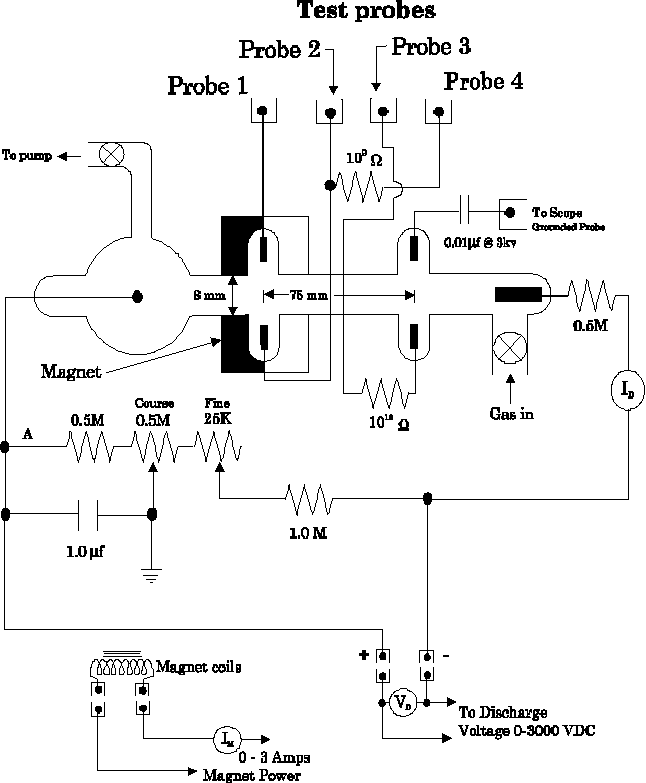
\includegraphics[width=0.8\linewidth]{images/DiagramAppartatus.png}}
\end{center}

\section{Hall Effect Magnet Power Circuit Schematic}

\begin{center}
    \href{http://experimentationlab.berkeley.edu/sites/default/files/images/MagnetReverseCiruit02.png}{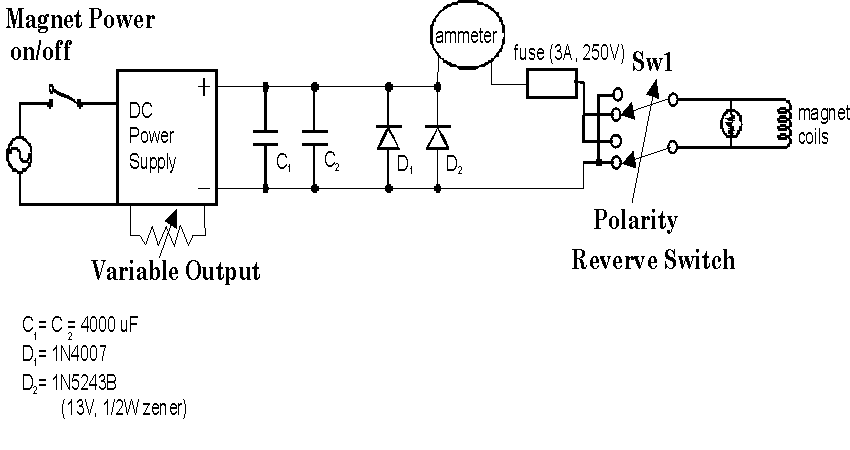
\includegraphics[width=0.8\linewidth]{images/MagnetReverseCiruit02.png}}
\end{center}

\section{References}
\label{sec:References}

\begin{enumerate}
    \item S. C. Brown, \href{http://experimentationlab.berkeley.edu/sites/default/files/Electrical-Discharges-In-Gases.pdf}{\textbf{Introduction to Electrical Discharges in Gases}}, Wiley, New York, (1965).
    
    \item Merle N. Hirsh and H. J. Oskam, \emph{Gaseous Electronics Vol.1}, \href{http://physics111.lib.berkeley.edu/Physics111/Reprints/HAL/Gaseous\%20Electronics_HirshnOskam\%20ch2.pdf}{\textbf{Chapter 2}}, Academic Press (1978).
    

    \item R. N. Franklin, \href{http://physics111.lib.berkeley.edu/Physics111/Reprints/HAL/01-Plasma\_Phenomena\_in\_Gas\_Discharges.pdf}{\textbf{Plasma Phenomena in Gas Discharges}}, Clarendon Press, Oxford (1976), page 48.

    \item C. Kittel, \href{http://physics111.lib.berkeley.edu/Physics111/Reprints/HAL/02-Intro\_to\_Solid\_State\_Physics.pdf}{\textbf{Introduction to Solid State Physics}}, 4th Ed., Wiley, New York (1971), pp. 287-289.

    \item C. Kittel and H. Kroemer, \href{http://physics111.lib.berkeley.edu/Physics111/Reprints/HAL/Charles_Kittel-Herbert_Kroemer-Thermal_Physics.pdf}{\textbf{Thermal Physics}}, Freeman, SFO (1980).

    \item P. Lorrain \& R. D. Corson , ``\href{http://physics111.lib.berkeley.edu/Physics111/Reprints/HAL/03-Electromagnetic\_Field\_and\_Waves.pdf}{\textbf{Electromagnetic Fields and Waves}}'', Section 7.3, pp. 299-301.

    \item L. Pekarek, ``\href{http://physics111.lib.berkeley.edu/Physics111/Reprints/HAL/05-Ionization_Waves.pdf}{\textbf{Ionization Waves (Striations) in a Discharge Plasma}}'', Soviet Physics Uspekhi 11, 188-208 (1968).

    \item F. Chen, \emph{Introduction to Plasma Physics and Controlled Fusion}, \href{http://physics111.lib.berkeley.edu/Physics111/Reprints/HAL/06-Intro\_to\_Plasma\_Physics\_CH1.pdf}{\textbf{Chapter 1}} \& \href{http://physics111.lib.berkeley.edu/Physics111/Reprints/HAL/06-Intro\_to\_Plasma\_Physics\_CH5.pdf}{\textbf{Chapter 5}}, Vol. 1, 2nd ed., Plenum Press (1984).

\end{enumerate}

\noindent Other reprints and reference materials can be found on the \href{http://physics111.lib.berkeley.edu/Physics111/Reprints/HAL/HAL\_index.html}{\textbf{Physics 111 Library Site}}

\end{document}
